\documentclass[a4paper]{article} 
\addtolength{\hoffset}{-2.25cm}
\addtolength{\textwidth}{4.5cm}
\addtolength{\voffset}{-3.25cm}
\addtolength{\textheight}{5cm}
\setlength{\parskip}{0pt}
\setlength{\parindent}{0in}

\usepackage[square,sort,comma,numbers]{natbib}
\usepackage{blindtext} % Package to generate dummy text
\usepackage{charter} % Use the Charter font
\usepackage[utf8]{inputenc} % Use UTF-8 encoding
\usepackage{microtype} % Slightly tweak font spacing for aesthetics
\usepackage{amsthm, amsmath, amssymb} % Mathematical typesetting
\usepackage{float} % Improved interface for floating objects
\usepackage{hyperref} % For hyperlinks in the PDF
\usepackage{graphicx, multicol} % Enhanced support for graphics
\usepackage{xcolor} % Driver-independent color extensions
\usepackage{pseudocode} % Environment for specifying algorithms in a natural way
\usepackage[mmddyy]{datetime} % Uses YEAR-MONTH-DAY format for dates

\usepackage{fancyhdr} % Headers and footers
\pagestyle{fancy} % All pages have headers and footers
\fancyhead{}\renewcommand{\headrulewidth}{0pt} % Blank out the default header
\fancyfoot[L]{} % Custom footer text
\fancyfoot[C]{} % Custom footer text
\fancyfoot[R]{\thepage} % Custom footer text
\newcommand{\note}[1]{\marginpar{\scriptsize \textcolor{red}{#1}}} % Enables comments in red on margin

\DeclareMathOperator*{\argmin}{arg\,min}

%----------------------------------------------------------------------------------------


%-------------------------------
%	TITLE VARIABLES (identify your work!)
%-------------------------------

\newcommand{\yourname}{Balthazar Neveu | Jamy Lafenetre}
\newcommand{\youremail}{balthazarneveu@gmail.com | jamy.lafenetre@ens-paris-saclay.fr}
\newcommand{\assignmentnumber}{6}

\begin{document}

%-------------------------------
%	TITLE SECTION (do not modify unless you really need to)
%-------------------------------
\fancyhead[C]{}
\hrule \medskip
\begin{minipage}{0.295\textwidth} 
\raggedright
\footnotesize
\yourname \hfill\\
\youremail
\end{minipage}
\begin{minipage}{0.4\textwidth} 
\centering 
\large 
Lab session \# \assignmentnumber\\ 
\normalsize 
NPM 2024\\ 
\end{minipage}
\begin{minipage}{0.295\textwidth} 
\raggedleft
\today\hfill\\
\end{minipage}
\medskip\hrule 
\bigskip




%-------------------------------
%	ASSIGNMENT CONTENT (add your responses)
%-------------------------------

\section*{Preliminary question: Ability of MLP to classify coordinates.}
\begin{figure}[H]
    \centering
    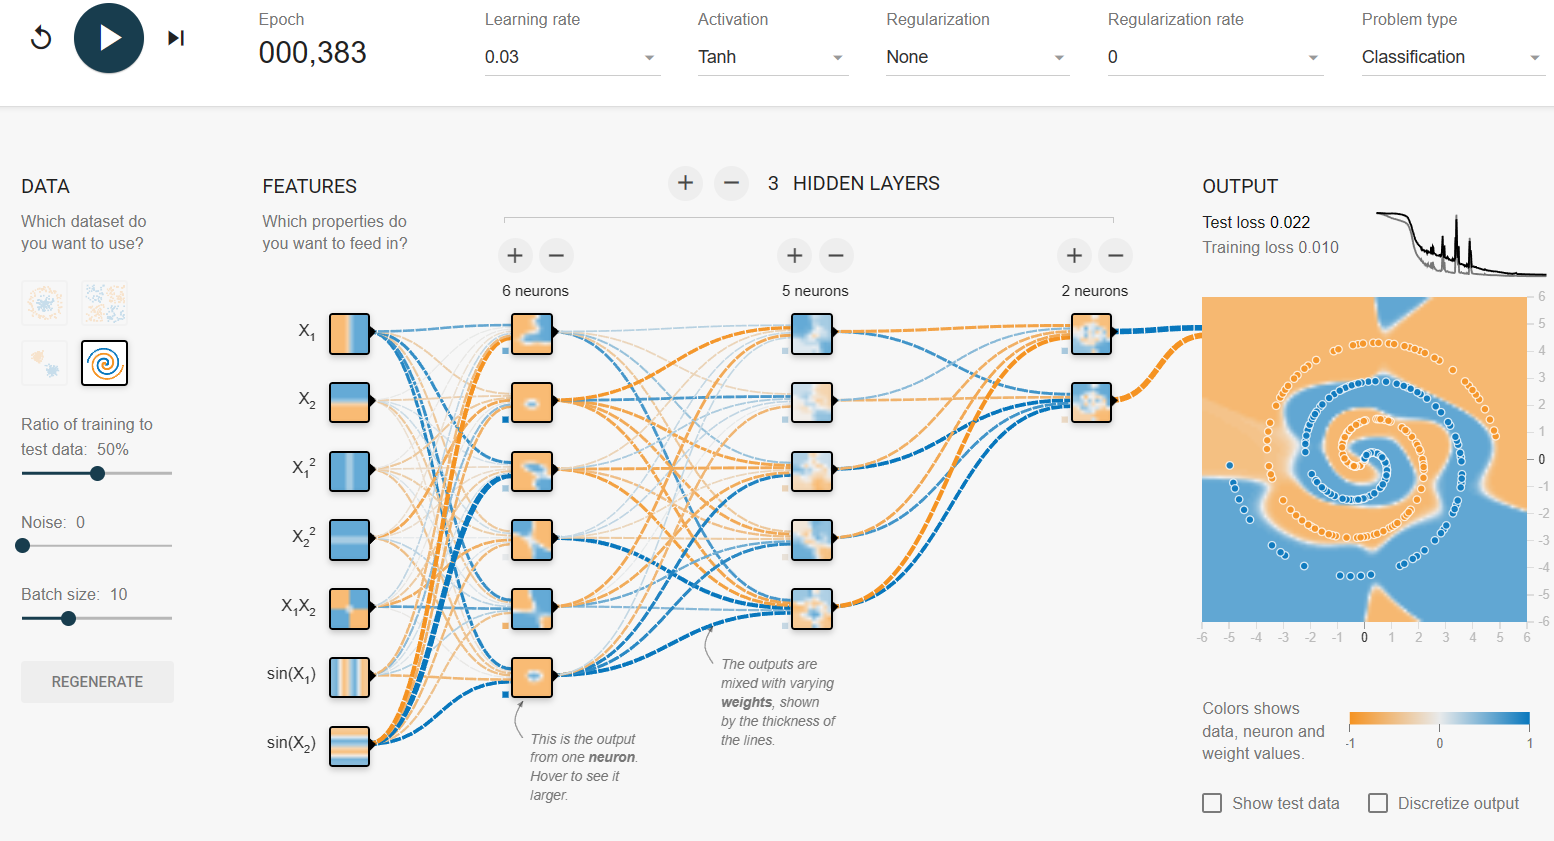
\includegraphics[width=0.8\textwidth]{figures/mlp_manual.png}
    \caption{Multi layer perceptron show the ability to  classify coordinates. We display parameters which led to good results on the spiral classification.}
    \label{fig:MPL_search}
\end{figure}

\begin{itemize}
    \item The Cybenko theorem of universal approximation states that we should be able to classify this point cloud with a single hidden layer with enough neurons. 
    \item When we use ReLu function, MLP outputs a piecewise linear function of the input coordinates.
    \item To classify the spiral points, the output logits may need to use the radius... which is possible to approximate with a very wide hidden layer.
    \item Hower instead of learning to appoximate $x^2 + y^2$ with a bunch of layers and ReLU to get the radius, we can directly inject it as an extra input.
    \item Introducing squared coordinates (and sinus embeddings) allows the model to output piecewise linear functions of more complex inputs features (a piecewise quadratic form if we consider the squared $x^2$ ).
    \item We note that finding the right architecture (depth and number of layers) is a matter of trial and error here.
\end{itemize}

We can see that eventually, we're able to find correct parameters which allow finding a shape which roughly match the spiral.   

Now the following lab session deals on how we classify 3D point clouds (e.g. unordered sets of points in 3D space). We will use a PointNet architecture to classify 3D point clouds.

\section*{Question 1}

We train our model on ModelNet40. It has 1.708M parameters. Using a learning rate of $10^{-}2$, we
are only able to reach an accuracy of $12\%$ after 75 epochs (convergence is achieved).

The accuracy of a random classifier would be $2.5\%$, so this result is not dramatic. 
However it cannot be considered a good classifier.
Please note that MLP considers that the order of the points matters (a list instead of a set) and therefore the output is not \textbf{permutation invariant}.
A detailed unitary test is available in the code (test\_pointnet.py to make sure that pointNet architecture is actually permutation invariant).


\section*{Question 2}
On ModelNet40, we reach an accuracy of $86\%$ after 75 epochs using a learning rate of $1e-3$.
These results are considerably higher than using a simple MLP. A Pointnet without Tnets can be used
like a satisfactory classifier.
Unlike the initial MLP, PointNet processes each point of the set separately until the max pooling operator is reached. Max pooling statisfies the permutation invariance.


\section*{Question 3}
On ModelNet40, we reach an accuracy of $84\%$ after 100 epochs using a learning rate of $5e-3$.
These results are slightly under what could be obtained without Tnet.
Our intuition is that by using TNet, network may learn to orient objects in a canonical way, which may not always the best way to classify them... it is almost like trying to counter-act the effect of augmentations.

\section*{Question 4}
We propose two sources of data augmentation. 
\begin{itemize}
    \item First, we apply three random scaling factors centered around 1 in the x, y and z direction. 
    \item Second, we remove a random proportion of the points (around $10\%$) and replace them by duplicating other points.
\end{itemize}
Using the same parameters as before, the impact of this data augmentation is not meaningful and seems to slightly hinder the accuracy.


\begin{figure}[H]
    \centering
    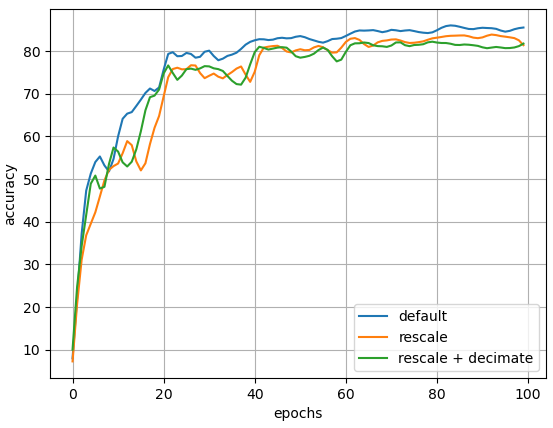
\includegraphics[width=0.5\textwidth]{figures/Q4.png}
    \caption{Impact on validation accuracy of our augmentations during PointNet training - seems like adding new augmentations sligtlty slowed down convergence and prevented to reach the best accuracy.}
    \label{fig:pointNet augmentations}
\end{figure}

\section*{Conclusion}
All evaluations conducted on ModelNet40 are summarized in Table \ref{tab:classification_results}. We can see that the PointNet architecture is able to classify 3D point clouds with a decent accuracy. However, the use of T-Net (promising idea on paper) does not seem to improve the results... nor data augmentation.
\begin{table}[H]
    \centering
    \begin{tabular}{|l|c|c|c|}
    \hline
    \textbf{Model} & \textbf{Learning Rate} & \textbf{Epochs} & \textbf{Accuracy} \\ \hline
    MLP (Not permutation invariant) & $10^{-2}$ & 75 & 12\% \\ \hline
    PointNet without T-Net & $10^{-3}$ & 75 & 86\% \\ \hline
    PointNet with T-Net & $5 \times 10^{-3}$ & 100 & 84\% \\ \hline
    PointNet with T-Net and Data Augmentation & $5. 10^{-3}$ & 100 & 83\% \\ \hline
    \end{tabular}
    \caption{Summary of Point Cloud Classification Results}
    \label{tab:classification_results}
\end{table}

Foreseen potential ideas for improvements include:
\begin{itemize}
    \item Add sinusoidal and quadratic embeddings of the coordinates into the input features.
    \item Interpretability of the PointNet architecture: visualize the points which were selected by the max pooling operator (find all max indexes and display the corresponding points in colors, we may find gain interpretability on how PointNet intuitively works).
\end{itemize}

\section*{Appendix: training curves}

    
\begin{figure}[H]
    \centering
    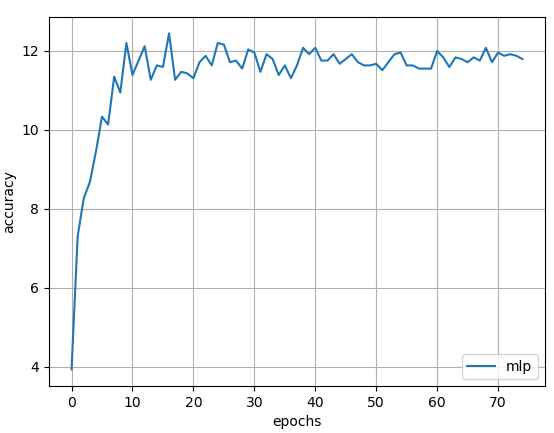
\includegraphics[width=0.5\textwidth]{figures/Q1.png}
    \caption{MLP accuracy during training}
    \label{fig:MLP}
\end{figure}

\begin{figure}[H]
    \centering
    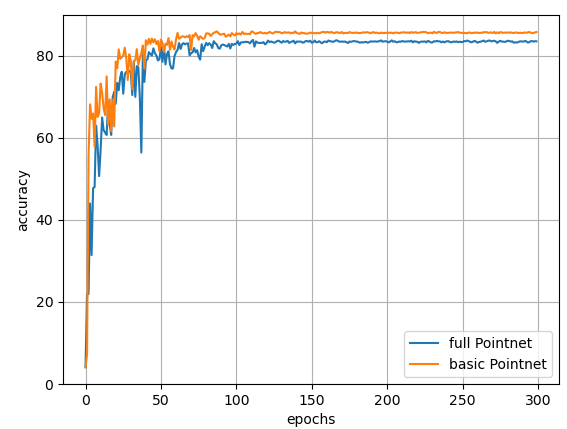
\includegraphics[width=0.5\textwidth]{figures/Q3.png}
    \caption{PointNet (no TNET vs TNET) + standard augmentations) validation accuracy during training}
    \label{fig:pointNet}
\end{figure}

\break


\section*{Appendix: T-NET validation}
To validate our TNET implementation, we create a simple synthetic object \ref{fig:validation_object}.
We then optimize (overfit) the TNET to "correct" the orientation of the object. Convergence is demonstrated in figure \ref{fig:validation_convergence_Tnet}. Please refer to the code check\_tnet.py for more details.

\begin{figure}[H]
    \centering
    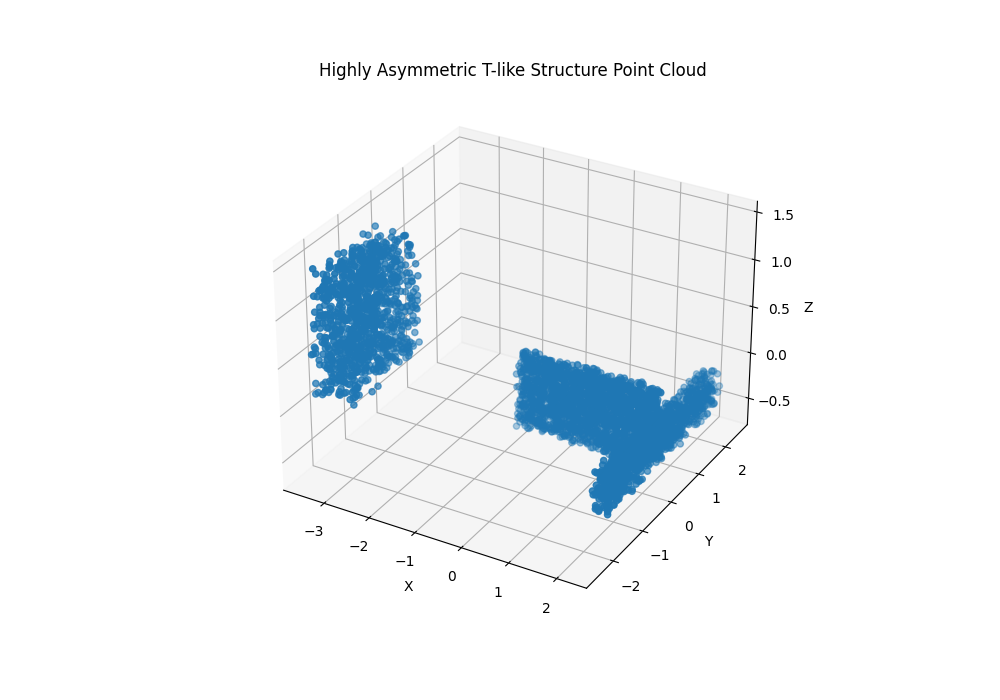
\includegraphics[width=0.2\textwidth]{figures/TNET_validation.png}
    \caption{The expected orientation of the object}
    \label{fig:validation_object}
\end{figure}

\begin{figure}[H]
    \centering
    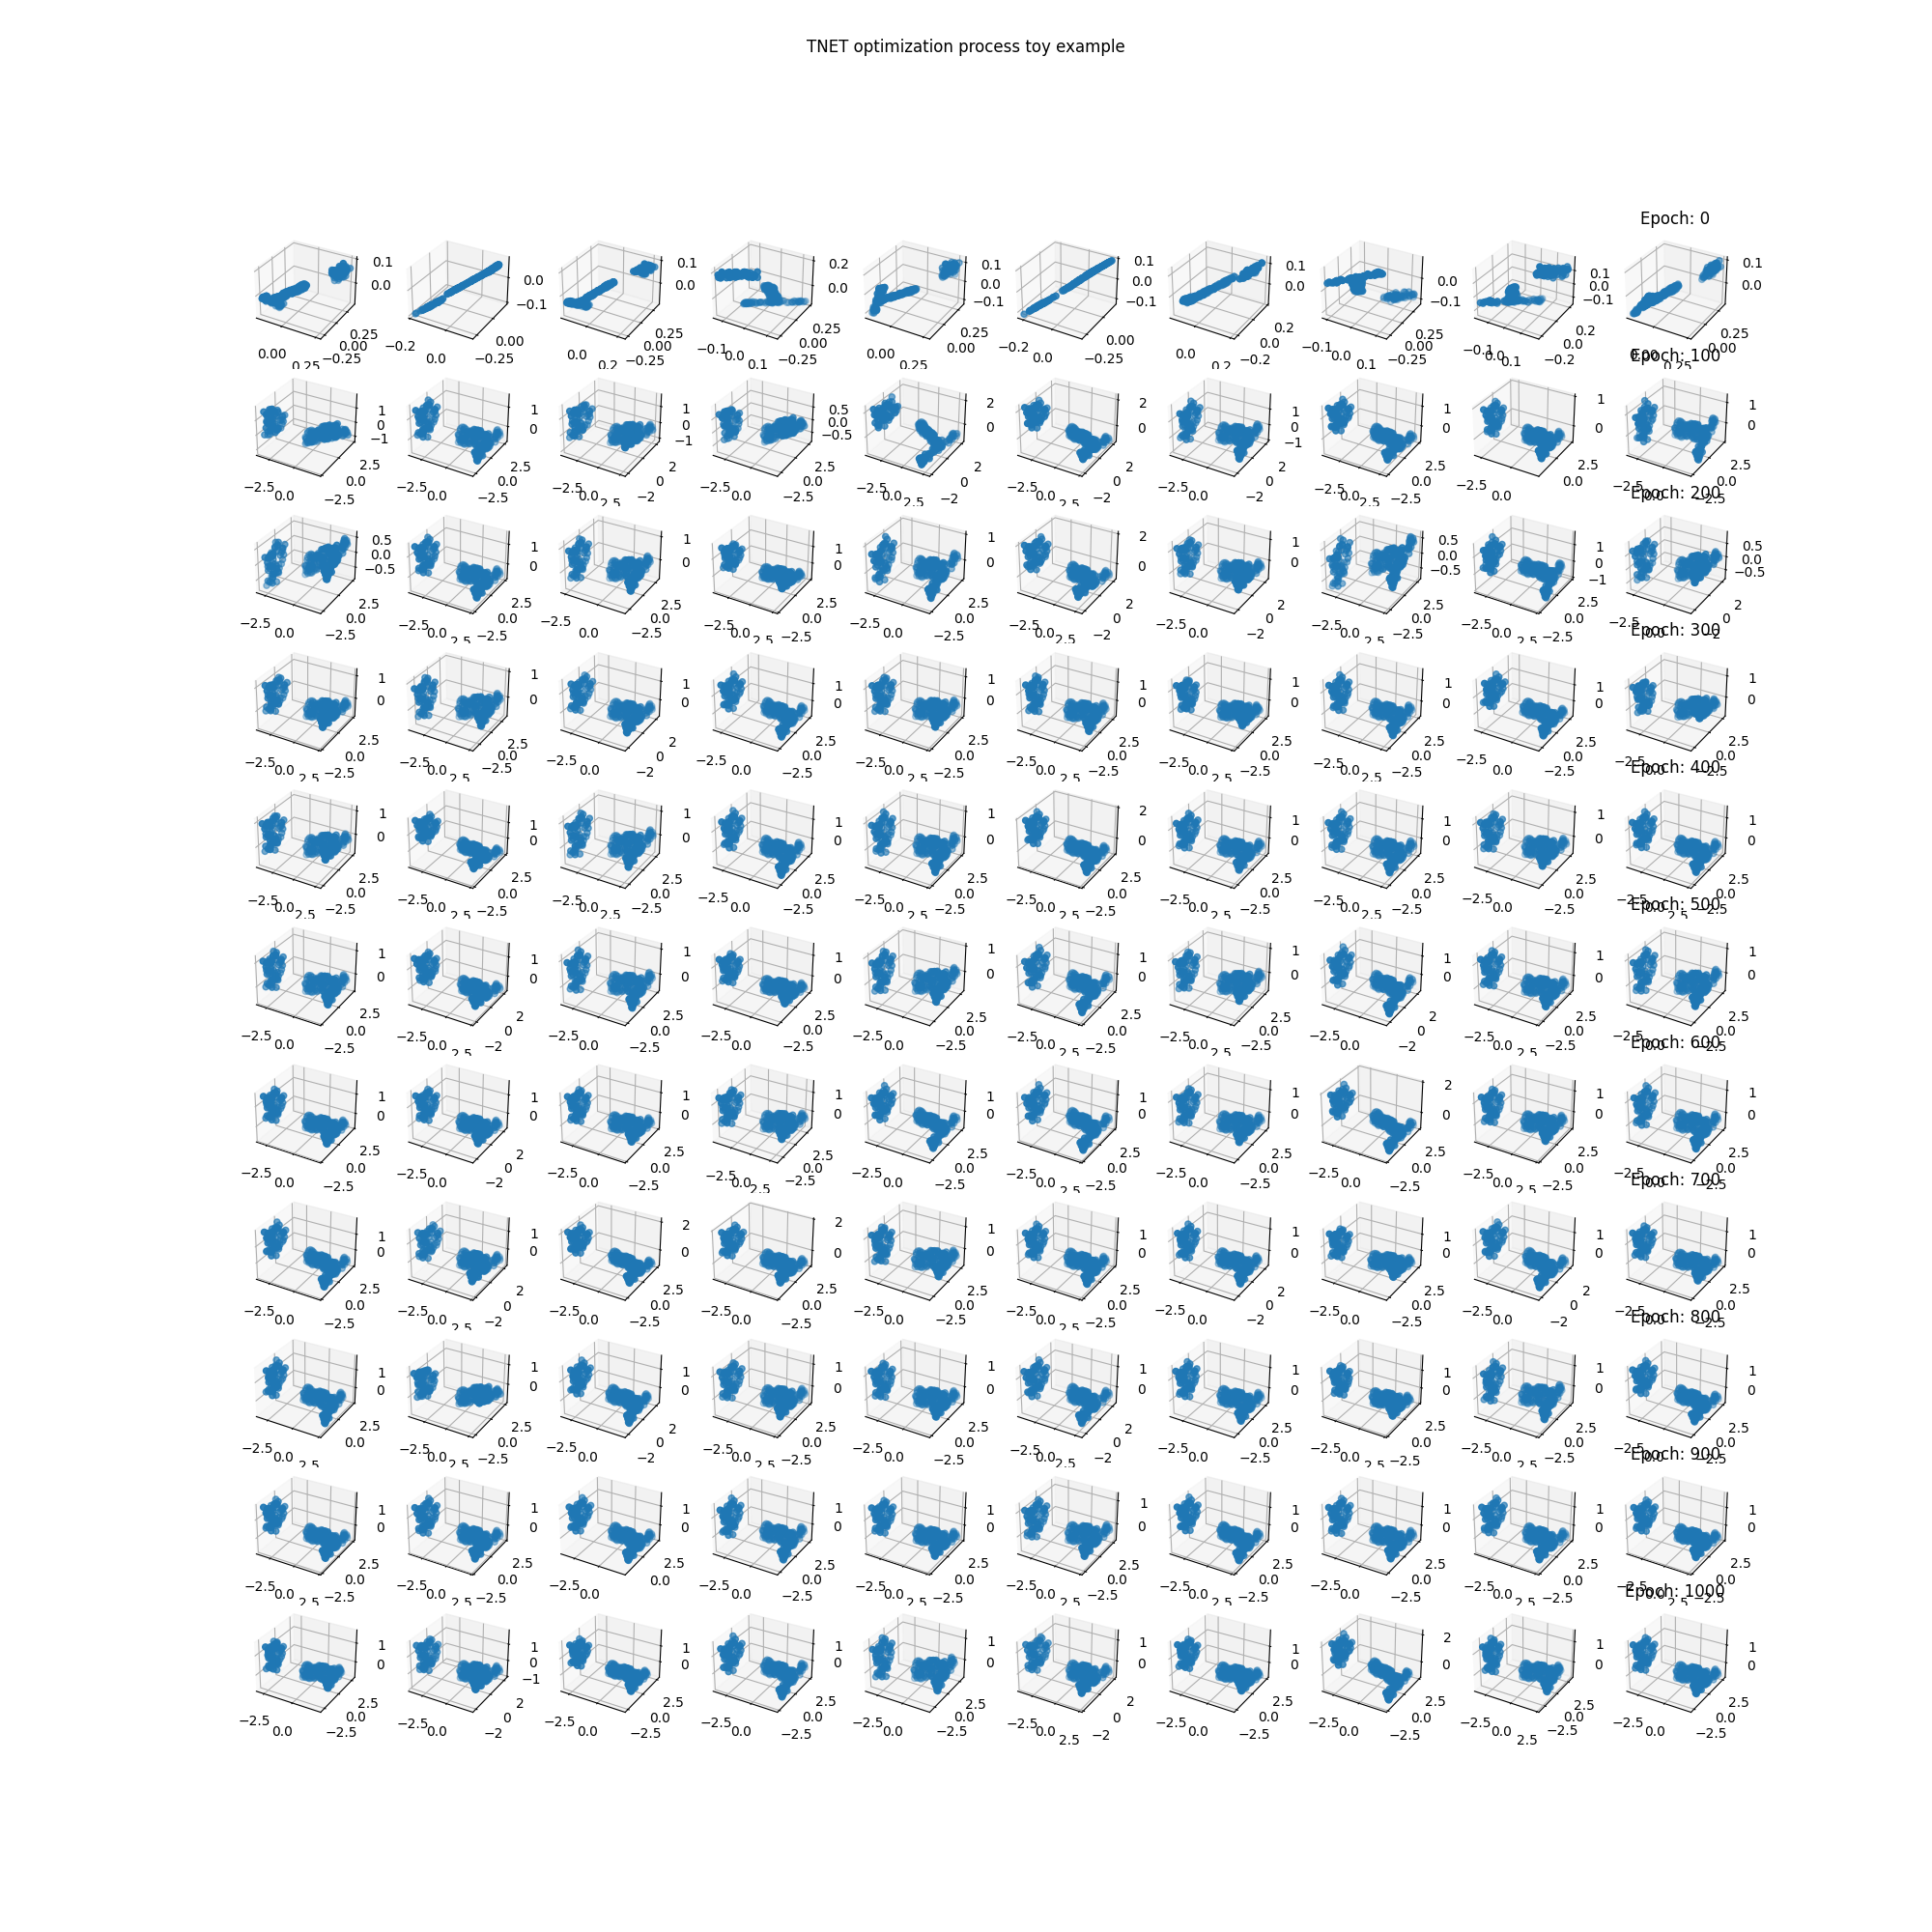
\includegraphics[width=1.\textwidth]{figures/TNET_optimization.png}
    \caption{Horizontally, we show 10 same random orientations of the object after being "corrected" by the TNET.
    Vertically, we see the convergence of the TNET across epochs. Here the optimization is performed on the predicted matrices directly and by optimizing the Froebenius norm of the difference between the predicted and expected matrices. We can see for instance that at the begining, the scales are not correct.
    }
    \label{fig:validation_convergence_Tnet}
\end{figure}

\textit{Please note that optimization could very well be performed on the predicted point cloud directly instead of the rotation matrices.}

\end{document}



